\documentclass[tikz,border=10pt]{standalone}
\usepackage{tkz-euclide} % 专门用于几何作图的宏包增强

\begin{document}
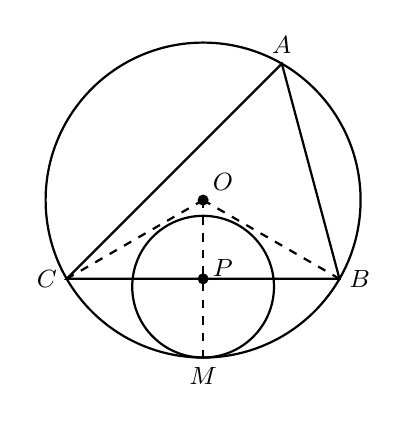
\begin{tikzpicture}[scale=2, font=\small]
    % 1. 定义基本参数
    % 设定大圆圆心 O 为原点，半径为 1
    \coordinate (O) at (0,0);
    \def\R{1}
    
    % 2. 定义三角形顶点坐标 (根据原图位置估算角度)
    \coordinate (A) at (60:\R);
    \coordinate (B) at (-30:\R);
    \coordinate (C) at (210:\R);
    
    % 3. 辅助计算：过 O 垂直于 BC 的垂足（即 BC 的中点，且位于对称轴上）
    \coordinate (P) at ($(B)!0.5!(C)$); % BC 中点
    % 延长 OP 交大圆于点 M
    \path (O) ; \pgfgetlastxy{\Ox}{\Oy}
    \coordinate (M) at (0,-1); % 根据图片，M 位于大圆的最底端
    
    % 4. 计算小圆 P 的参数
    % 假设小圆圆心在 P，且与大圆内切于 M（根据图示 P 是垂足点）
    % 小圆半径 r 为 PM 的长度
    \path (P); \pgfgetlastxy{\Px}{\Py}
    \def\smallradius{0.41} % 根据视觉比例调整
    \coordinate (P_center) at (0, -0.59); % 小圆圆心
    
    % 5. 绘制图形
    % 绘制外接大圆
    \draw[thick] (O) circle (\R);
    
    % 绘制三角形 ABC
    \draw[thick] (A) -- (B) -- (C) -- cycle;
    
    % 绘制小圆 (以 P 为圆心在视觉上更靠近 BC 和弧 M 之间)
    \draw[thick] (0,-0.55) circle (0.45); % 调整小圆位置和大小以匹配原图比例
    
    % 6. 绘制辅助线 (虚线)
    \draw[dashed, thick] (O) -- (C);
    \draw[dashed, thick] (O) -- (B);
    \draw[dashed, thick] (O) -- (0,-1); % 垂直平分线 O-P-M
    
    % % 7. 标注特殊点 (打点)
     \foreach \p in {O, P}
    \fill (\p) circle (1pt);
    % \fill (0,-0.55) circle (1pt); % 小圆圆心

    % 8. 文字标签
    \node[above] at (A) {$A$};
    \node[right] at (B) {$B$};
    \node[left] at (C) {$C$};
    \node[above right] at (O) {$O$};
    \node[above right] at (0,-0.55) {$P$};
    \node[below] at (0,-1) {$M$};

\end{tikzpicture}
\end{document}